\iffalse
\documentclass[12pt]{article}
\usepackage{graphicx}
\usepackage[none]{hyphenat}
\usepackage{graphicx}
\usepackage{listings}
\usepackage[english]{babel}
\usepackage{graphicx}
\usepackage{caption} 
\usepackage{booktabs}
\usepackage{array}
\usepackage{amssymb} % for \because
\usepackage{amsmath}   % for having text in math mode
\usepackage{extarrows} % for Row operations arrows
\usepackage{listings}
\lstset{
  frame=single,
  breaklines=true
}
\usepackage{hyperref}
  
%Following 2 lines were added to remove the blank page at the beginning
\usepackage{atbegshi}% http://ctan.org/pkg/atbegshi
\AtBeginDocument{\AtBeginShipoutNext{\AtBeginShipoutDiscard}}


%New macro definitions
\newcommand{\mydet}[1]{\ensuremath{\begin{vmatrix}#1\end{vmatrix}}}
\providecommand{\brak}[1]{\ensuremath{\left(#1\right)}}
\providecommand{\norm}[1]{\left\lVert#1\right\rVert}
\newcommand{\solution}{\noindent \textbf{Solution: }}
\newcommand{\myvec}[1]{\ensuremath{\begin{pmatrix}#1\end{pmatrix}}}
\providecommand{\abs}[1]{\left\vert#1\right\vert}
\let\vec\mathbf

\begin{document}

\begin{center}
\title{\textbf{Equation  of Line}}
\date{\vspace{-5ex}} %Not to print date automatically
\maketitle
\end{center}
\setcounter{page}{1}

\section{11$^{th}$ Maths - Chapter 10}
This is Problem-4 from Exercise 10.3
\begin{enumerate}
		\fi
\item Find the distance of the point $(-1,1)$ from the line $12\brak{x+6} = 5\brak{y-2}$. 
	\\
\solution 
\begin{enumerate}
\item The equation of the line is $12\brak{x+6} = 5\brak{y-2}$. Rearranging the equation, 
\begin{align}
12x-5y = -10-72 \\
12x-5y = -82
\end{align}

This can be equated to

\begin{align}
	\label{eq:11/10/3/4/2Dline}
	\vec{n}^\top\vec{x} = c 
\end{align}
\begin{align}
	\text{ where }
		\vec{n} = \myvec{
	  12 \\
	  -5 
	  } ,   c = -82 
\end{align}
		We need to compute the distance from a point $\vec{P}\myvec{-1 \\ 1}$ to the line. 
Without loss of generality, let $\vec{A}$ be the foot of the perpendicular from $\vec{P}$ to the line in Equation \eqref{eq:11/10/3/4/2Dline}. 
The equation of the normal to Equation \eqref{eq:11/10/3/4/2Dline} can then be expressed as 

\begin{align}
	\label{eq:11/10/3/4/dir_line_normal_dist}
	\vec{x} &= \vec{A} + \lambda \vec{n}
	\\
	\implies 
	\label{eq:11/10/3/4/dir_line_normal_dist_pa}
	\vec{P}- \vec{A} &=  \lambda \vec{n}
\end{align}

$\because \vec{P}$ lies on 
		\eqref{eq:11/10/3/4/dir_line_normal_dist}.
From the above, the desired distance can be expressed as 

\begin{align}
	\label{eq:11/10/3/4/dir_line_normal_dist_pa_d}
d = 	\norm{\vec{P}- \vec{A}}= \abs{\lambda} \norm{\vec{n}}
\end{align}

From 
	\eqref{eq:11/10/3/4/dir_line_normal_dist_pa},

\begin{align}
	\vec{n}^{\top}
	\brak{\vec{P}- \vec{A}} &=  \lambda \vec{n}^{\top}\vec{n} = \lambda\norm{\vec{n}}^2
	\\
	\implies \abs{\lambda}&= \frac{\abs{\vec{n}^{\top}
	\brak{\vec{P}- \vec{A}}}}{\norm{\vec{n}}^2} 
\end{align}

Substituting the above in \eqref{eq:11/10/3/4/dir_line_normal_dist_pa_d} and using the fact that

\begin{align}
   \vec{n}^{\top}\vec{A} = c
\end{align}

from 	\eqref{eq:11/10/3/4/2Dline}, yields 

\begin{align}
	\label{eq:11/10/3/4/line_dist_2d}
	d = \frac{\abs{   \vec{n}^{\top}\vec{P}-c }}{\norm{\vec{n}}}	
\end{align}

\begin{align}
	= \frac{\abs{  \myvec{12 & -5 }\myvec{-1 \\ 1}-\brak{-82} }}{\sqrt{12^2+\brak{-5}^2}} \\	
	= \frac{\abs{  -17 + 82 }}{\sqrt{169}}	
	= \frac{\abs{65 }}{13}
	= 5 \text{ units }
\end{align}
\item The foot of the perpendicular from $\vec{P}\myvec{-1 \\ 1}$ to line in \eqref{eq:11/10/3/4/2Dline} is expressed as
\begin{align}
	\label{eq:11/10/3/4/foot_of_perpendicular}
	\myvec{\vec{m} & \vec{n}}^\top\vec{A} &= 
	   \myvec{
              \vec{m}^\top\vec{P}\\
	      c
	      }
\end{align}
where $\vec{m}$ is the direction vector of the given line
\begin{align}
    \because \vec{n} = \myvec{ 12 \\ -5},   
    \vec{m} = \myvec{ 5 \\ 12} \\ 
	\eqref{eq:11/10/3/4/foot_of_perpendicular} \implies \myvec{5&12 \\ 12 & -5}\vec{A} &= \myvec{\myvec{5 & 12}\myvec{-1 \\ 1}\\ -82} \\
	\label{eq:11/10/3/4/sysEq1}
	\myvec{5&12 \\ 12 & -5}\vec{A} &= \myvec{7 \\ -82} 
\end{align}	
The augmented matrix for the system equations in \eqref{eq:11/10/3/4/sysEq1} is expressed as
\begin{align}
	\myvec{5&12 & \vrule & 7 \\ 12 & -5 & \vrule & -82} 
\end{align}
Performing sequence of row operations to transform into RREF form
\begin{align}
        \xleftrightarrow[]{{R_2\rightarrow R_2-\frac{12}{5}R_1}}  
	\myvec{5&12 & \vrule & 7 \\ 0 & -\frac{169}{5} & \vrule & -\frac{494}{5}} \\
	\xleftrightarrow[{R_1\rightarrow \frac{1}{5}}R_1]{{R_2\rightarrow \frac{-5}{169}R_2}}  
	\myvec{1 & \frac{12}{5} & \vrule & \frac{7}{5} \\ 0 & 1 & \vrule & \frac{38}{13}} \\
	\xleftrightarrow[]{{R_1\rightarrow R_1-\frac{12}{5}R_2}}  
	\myvec{1 & 0 & \vrule & -\frac{73}{13} \\ 0 & 1 & \vrule & \frac{38}{13}} \\
	\vec{A} = \myvec{ -\frac{73}{13} \\ \frac{38}{13} }
\end{align}
\end{enumerate}
The desired line and the perpendicular line from $\vec{P}$ is shown as in Fig. \ref{fig:11/10/3/4/Fig1}
\begin{figure}[!h]
	\begin{center}
		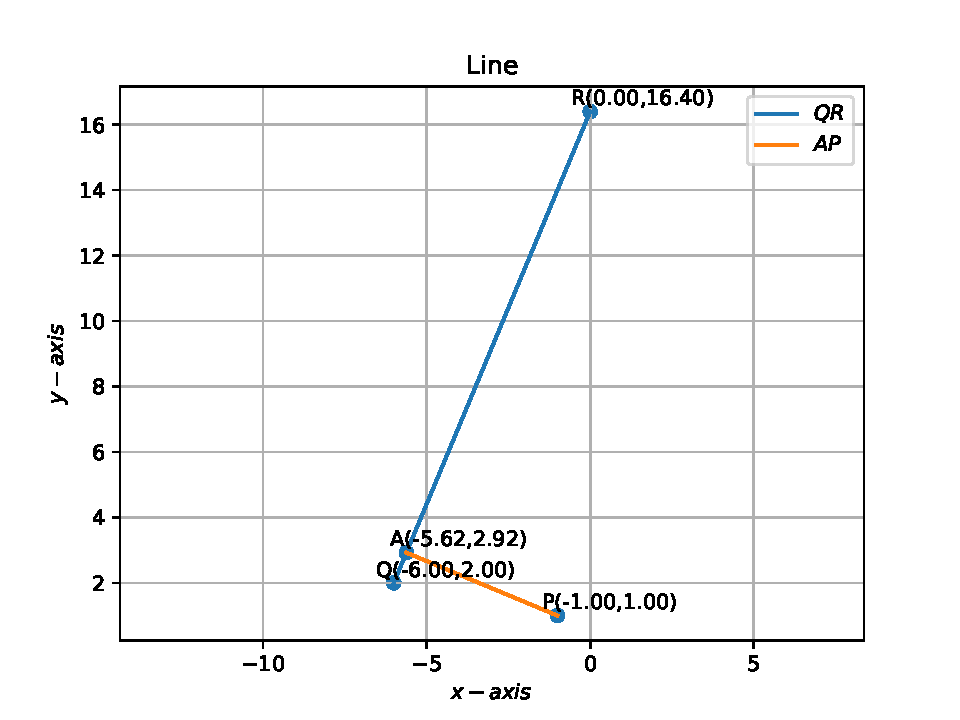
\includegraphics[width=\columnwidth]{chapters/11/10/3/4/figs/problem4.pdf}
	\end{center}
\caption{}
\label{fig:11/10/3/4/Fig1}
\end{figure}
